\subsection{Tahapan dan Implementasi}

Tahapan implementasi aplikasi Jatidiri dilakukan berdasarkan metode Prototype yang telah dijelaskan pada BAB III. Secara umum, tahapan implementasi terdiri dari beberapa langkah utama, yaitu:

1. Analisis Desain Figma

Pada tahap awal, desain antarmuka pengguna (UI/UX) yang telah dibuat di Figma dianalisis untuk memahami struktur halaman, komponen UI, navigasi, warna, tipografi, serta interaksi pengguna.

2. Pembuatan Struktur Proyek Flutter

Struktur proyek Flutter dibuat dengan pendekatan modular, yaitu memisahkan setiap halaman aplikasi ke dalam file dan folder yang berbeda untuk memudahkan pengembangan dan pemeliharaan kode.

3. Implementasi Antarmuka Pengguna (UI) di Flutter

Desain dari Figma kemudian diterjemahkan ke dalam komponen Flutter menggunakan widget seperti Scaffold, Container, Column, Row, ListView, Card, dan Button. Implementasi difokuskan pada:

a. Halaman Splash Screen

b. Halaman Walkthrough

c. Halaman Register

d. Halaman Login

e. Halaman Forgot Password

f. Halaman Survei

g. Halaman Home

h. Halaman Test

i. Halaman Detail Tes

j. Halaman Komunitas

4. Pengujian dan Penyempurnaan

Setelah setiap halaman diimplementasikan, dilakukan pengujian internal untuk memastikan kesesuaian tampilan dengan desain Figma. Jika ditemukan perbedaan atau masalah, dilakukan perbaikan sebelum melanjutkan ke tahap berikutnya.


\subsection{Hasil Implementasi}

Hasil implementasi aplikasi Jatidiri ditampilkan dalam bentuk halaman-halaman utama sebagai berikut:

\subsubsection{Halaman Splash Screen}

Halaman awal aplikasi yang menampilkan logo atau branding Jatidiri sebelum masuk ke aplikasi utama.

\begin{figure}[htbp]
    \centering
    % Splash Screen 1
    
\includegraphics[width=0.3\textwidth]{figures/splashscreen1.png}
    \caption{Splash Screen 1}
    \label{fig:Splash Screen 1}
\end{figure}
\begin{figure}[htbp]
    \centering
    % Splash Screen 2
    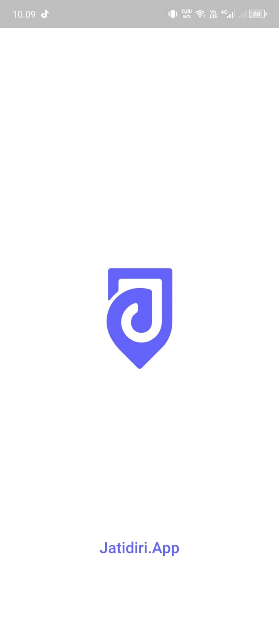
\includegraphics[width=0.3\textwidth]{figures/splashcreen2.png}
    \caption{Splash Screen 2}
    \label{fig:Splash Screen 2}
\end{figure}

\subsubsection{Halaman Walkthrough}

Halaman pengenalan fitur aplikasi untuk pengguna baru, berisi beberapa slide informasi.

\begin{figure}[htbp]
    \centering
    % Walkthrough 1
    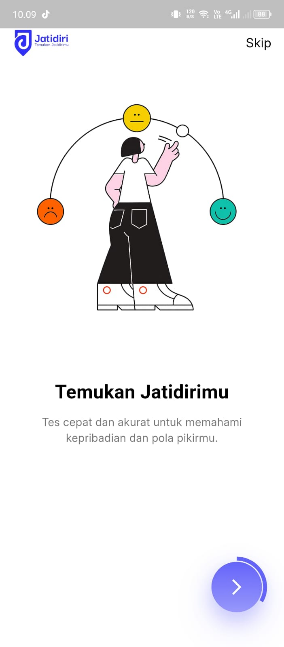
\includegraphics[width=0.3\textwidth]{figures/walktrough1.png}
    \caption{Walkthrough 1}
    \label{fig:Walkthrough 1}
\end{figure}

\begin{figure}[htbp]
    \centering
    % Walkthrough 2
    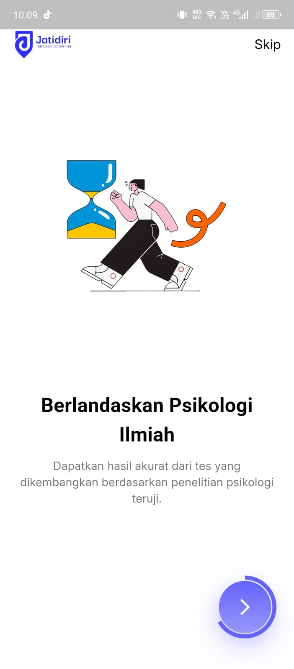
\includegraphics[width=0.3\textwidth]{figures/walktrough2.png}
    \caption{Walkthrough 2}
    \label{fig:Walkthrough 2}
\end{figure}

\begin{figure}[htbp]
    \centering
    % Walkthrough 3
    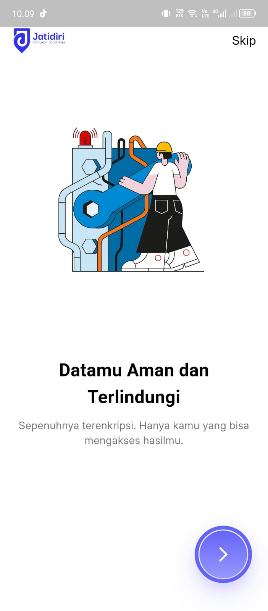
\includegraphics[width=0.3\textwidth]{figures/walktrough3.png}
    \caption{Walkthrough 3}
    \label{fig:Walkthrough 3}
\end{figure}

\begin{figure}[htbp]
    \centering
    % Walkthrough 4
    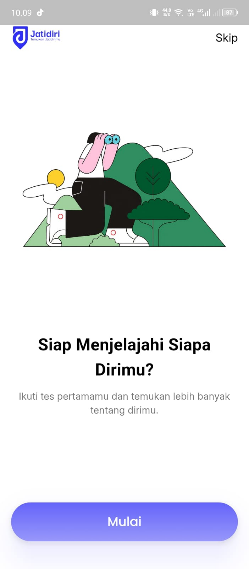
\includegraphics[width=0.3\textwidth]{figures/walktrough4.png}
    \caption{Walkthrough 4}
    \label{fig:Walkthrough 4}
\end{figure}


\subsubsection{Halaman Register}

Halaman pendaftaran akun pengguna dengan input seperti nama, email, password, tempat dan tanggal lahir.

\begin{figure}[htbp]
    \centering
    % Register 1
    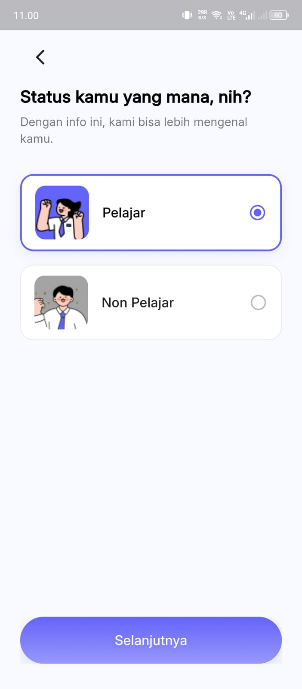
\includegraphics[width=0.3\textwidth]{figures/register1.png}
    \caption{Register 1}
    \label{fig:Register 1}
\end{figure}

\begin{figure}[htbp]
    \centering
    % Register 2
    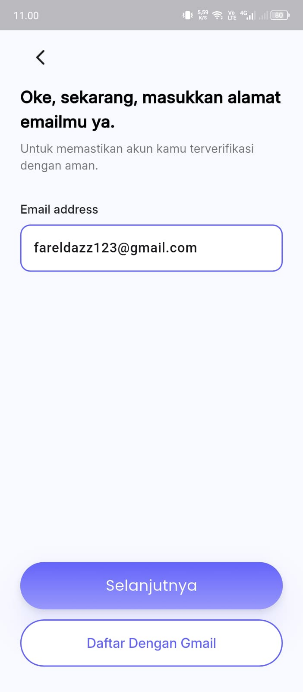
\includegraphics[width=0.3\textwidth]{figures/register2.png}
    \caption{Register 2}
    \label{fig:Register 2}
\end{figure}

\begin{figure}[htbp]
    \centering
    % Register 3
    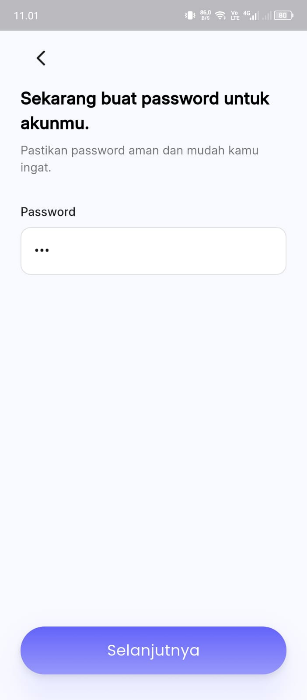
\includegraphics[width=0.3\textwidth]{figures/register3.png}
    \caption{Register 3}
    \label{fig:Register 3}
\end{figure}

\begin{figure}[htbp]
    \centering
    % Register 4
    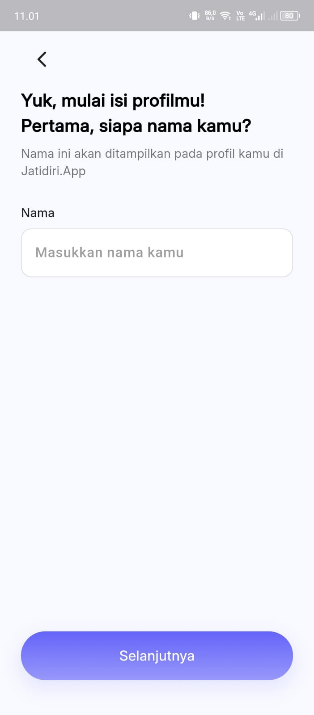
\includegraphics[width=0.3\textwidth]{figures/register4.png}
    \caption{Register 4}
    \label{fig:Register 4}
\end{figure}

\begin{figure}[htbp]
    \centering
    % Register 5
    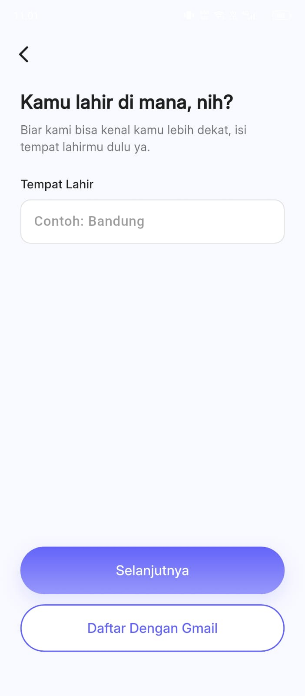
\includegraphics[width=0.3\textwidth]{figures/register5.png}
    \caption{Register 5}
    \label{fig:Register 5}
\end{figure}

\begin{figure}[htbp]
    \centering
    % Register 6
    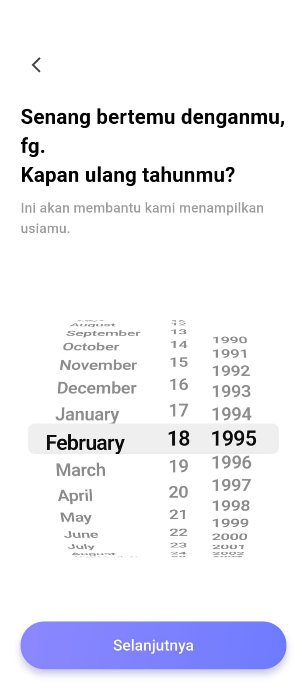
\includegraphics[width=0.3\textwidth]{figures/register6.png}
    \caption{Register 6}
    \label{fig:Register 6}
\end{figure}


\subsubsection{Halaman Login}

Halaman autentikasi pengguna untuk masuk ke aplikasi.

\begin{figure}[htbp]
    \centering
    % Login
    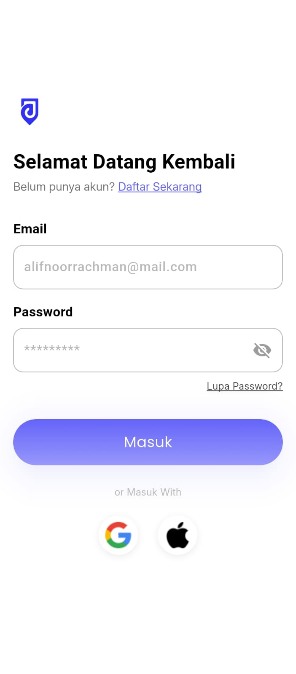
\includegraphics[width=0.3\textwidth]{figures/login.png}
    \caption{Login}
    \label{fig:Login}
\end{figure}


\subsubsection{Halaman Forgot Password}

Halaman pemulihan akun untuk pengguna yang lupa kata sandi.

\begin{figure}[htbp]
    \centering
    % Forgot Password 1
    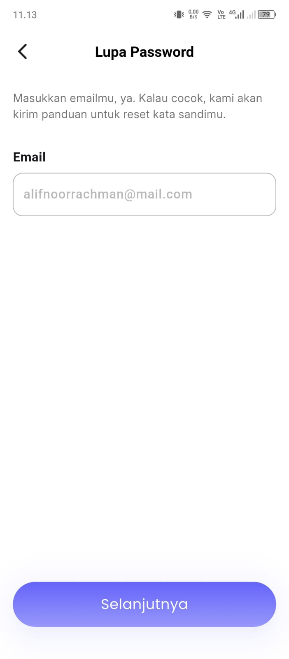
\includegraphics[width=0.3\textwidth]{figures/forgotpass1.png}
    \caption{Forgot Password 1}
    \label{fig:Forgot Password 1}
\end{figure}

\begin{figure}[htbp]
    \centering
    % Forgot Password 2
    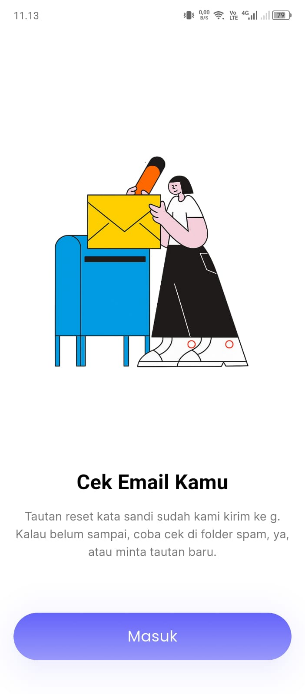
\includegraphics[width=0.3\textwidth]{figures/forgotpass2.png}
    \caption{Forgot Password 2}
    \label{fig:Forgot Password 2}
\end{figure}


\subsubsection{Halaman Survei}

Halaman survei awal yang harus diisi pengguna setelah login untuk menyesuaikan rekomendasi tes.

\begin{figure}[htbp]
    \centering
    % Survei 1
    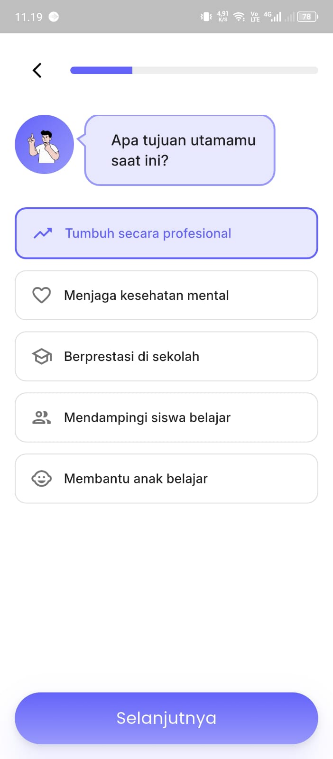
\includegraphics[width=0.3\textwidth]{figures/survei1.png}
    \caption{Survei 1}
    \label{fig:Survei 1}
\end{figure}

\begin{figure}[htbp]
    \centering
    % Survei 2
    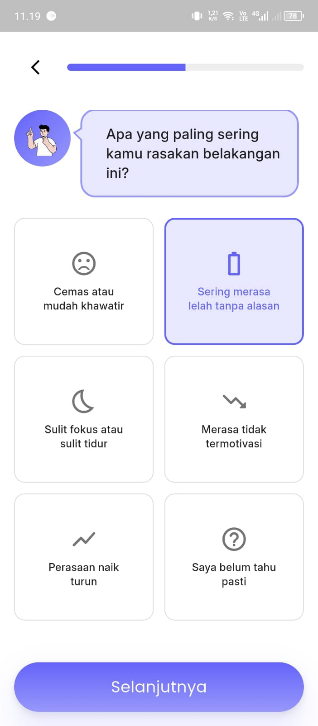
\includegraphics[width=0.3\textwidth]{figures/survei2.png}
    \caption{Survei 2}
    \label{fig:Survei 2}
\end{figure}

\begin{figure}[htbp]
    \centering
    % Survei 3
    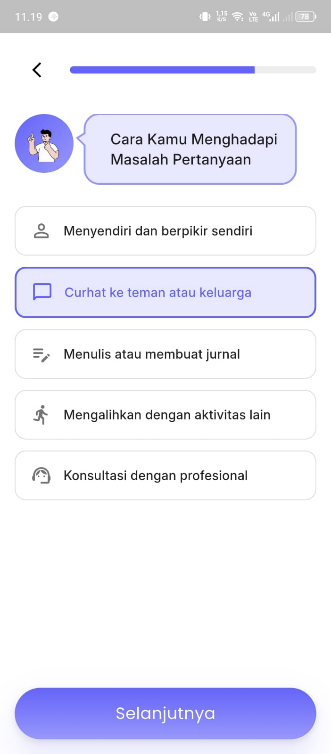
\includegraphics[width=0.3\textwidth]{figures/survei3.png}
    \caption{Survei 3}
    \label{fig:Survei 3}
\end{figure}

\begin{figure}[htbp]
    \centering
    % Survei 4
    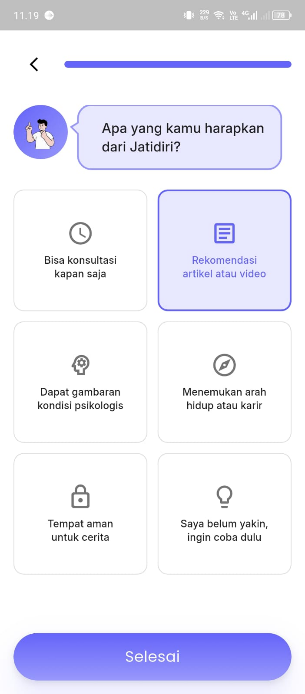
\includegraphics[width=0.3\textwidth]{figures/survei4.png}
    \caption{Survei 4}
    \label{fig:Survei 4}
\end{figure}


\subsubsection{Halaman Home}

Halaman utama aplikasi yang menampilkan profil, paket tes, kategori tes, dan history tes.

\begin{figure}[htbp]
    \centering
    % Home 1
    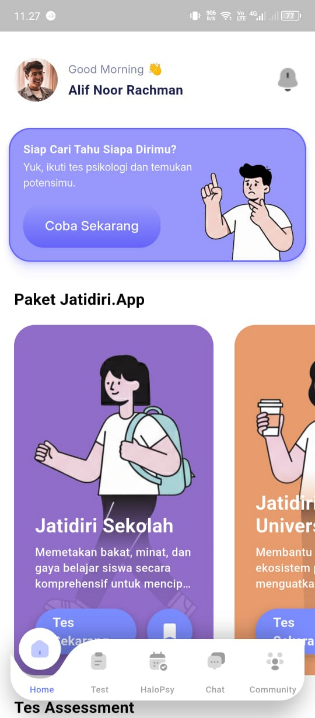
\includegraphics[width=0.3\textwidth]{figures/home1.png}
    \caption{Home 1}
    \label{fig:Home 1}
\end{figure}

\begin{figure}[htbp]
    \centering
    % Home 2
    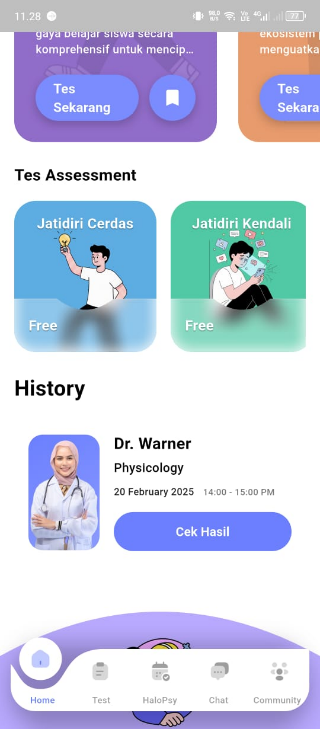
\includegraphics[width=0.3\textwidth]{figures/home2.png}
    \caption{Home 2}
    \label{fig:Home 2}
\end{figure}


\subsubsection{Halaman Test}

Menampilkan daftar tes, paket tes, dan hasil tes.

\begin{figure}[htbp]
    \centering
    % Test
    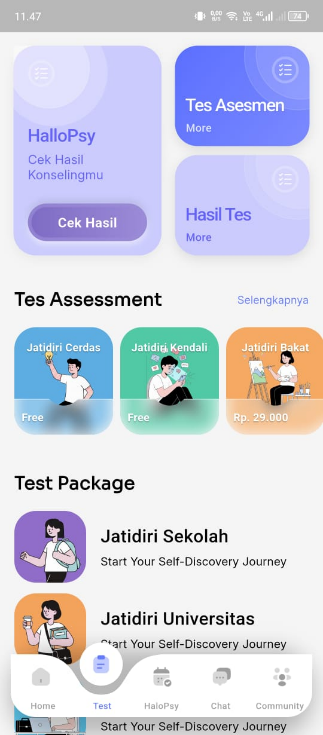
\includegraphics[width=0.3\textwidth]{figures/test.png}
    \caption{Test}
    \label{fig:Test}
\end{figure}


\subsubsection{Halaman Setiap Tes}

Setiap tes (misalnya tes kecerdasan, kecemasan, stres, dan lainnya) memiliki halaman khusus yang berisi pertanyaan dan pilihan jawaban.

\begin{figure}[htbp]
    \centering
    % Tes Bahagia 1
    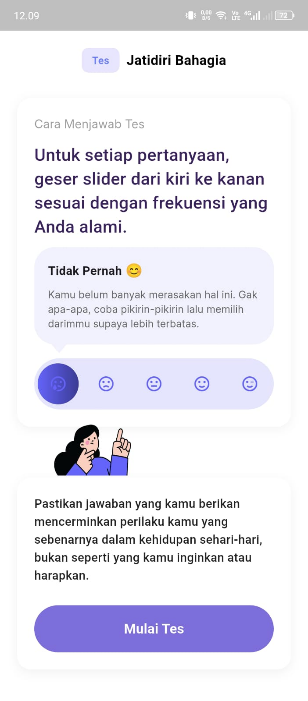
\includegraphics[width=0.3\textwidth]{figures/tesbahagia1.png}
    \caption{Tes Bahagia 1}
    \label{fig:TTes Bahagia 1}
\end{figure}

\begin{figure}[htbp]
    \centering
    % Tes Bahagia 2
    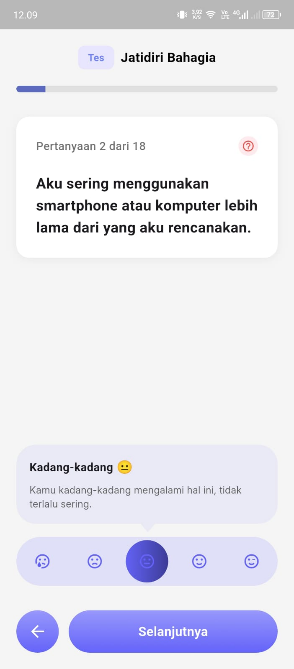
\includegraphics[width=0.3\textwidth]{figures/tesbahagia2.png}
    \caption{Tes Bahagia 2}
    \label{fig:TTes Bahagia 2}
\end{figure}

\begin{figure}[htbp]
    \centering
    % Tes Bahagia 3
    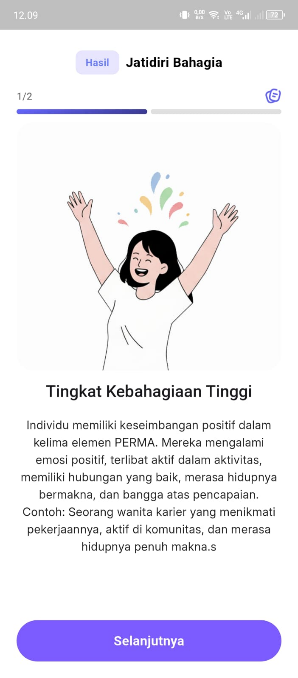
\includegraphics[width=0.3\textwidth]{figures/tesbahagia3.png}
    \caption{Tes Bahagia 3}
    \label{fig:TTes Bahagia 3}
\end{figure}

\begin{figure}[htbp]
    \centering
    % Tes Bahagia 4
    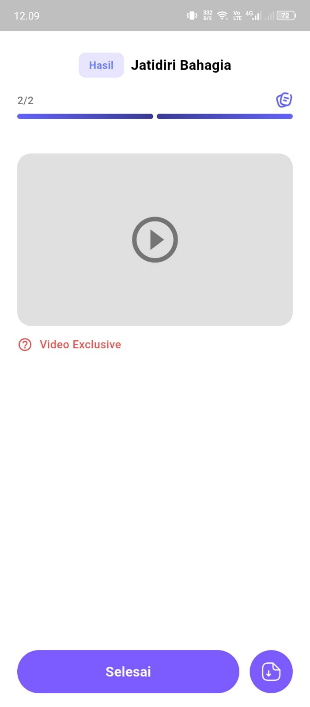
\includegraphics[width=0.3\textwidth]{figures/tesbahagia4.png}
    \caption{Tes Bahagia 4}
    \label{fig:TTes Bahagia 4}
\end{figure}


\subsubsection{Halaman Komunitas}

Halaman interaksi antar pengguna dalam aplikasi, pengguna juga dapat membuat komunitas masing-masing di dalam aplikasi ini.

\begin{figure}[htbp]
    \centering
    % Komunitas 1
    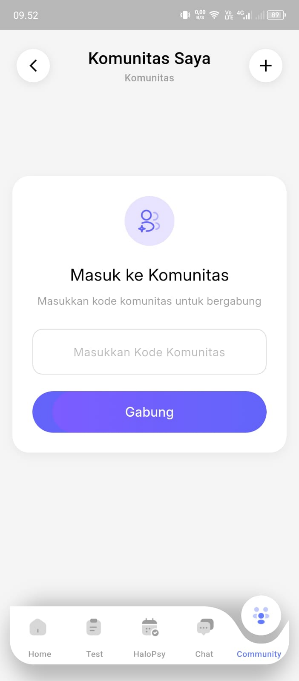
\includegraphics[width=0.3\textwidth]{figures/komunitas1.png}
    \caption{Komunitas 1}
    \label{fig:Komunitas 1}
\end{figure}

\begin{figure}[htbp]
    \centering
    % Komunitas 2
    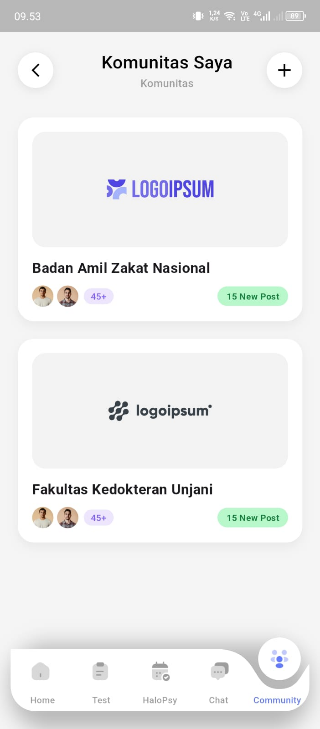
\includegraphics[width=0.3\textwidth]{figures/komunitas2.png}
    \caption{Komunitas 2}
    \label{fig:Komunitas 2}
\end{figure}

\begin{figure}[htbp]
    \centering
    % Komunitas 3
    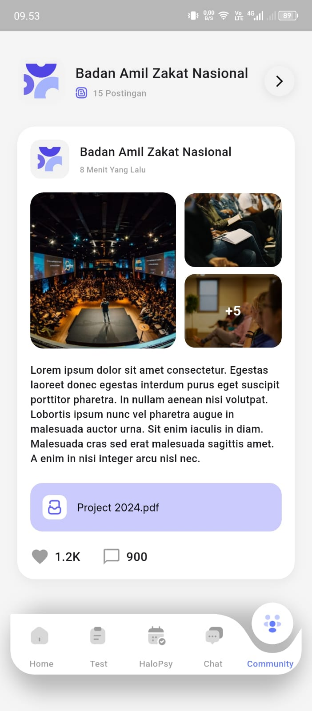
\includegraphics[width=0.3\textwidth]{figures/komunitas3.png}
    \caption{Komunitas 3}
    \label{fig:Komunitas 3}
\end{figure}


\subsection{Pengujian}

\subsubsection{Tujuan Pengujian}

a. Memastikan semua halaman dapat diakses dengan benar.

b. Memastikan navigasi antar halaman berfungsi.

c. Memastikan tombol dan input bekerja sesuai harapan.


\subsubsection{Skenario Pengujian}

\begin{table}[h!]
\centering
\caption{Tabel Pengujian Black Box}
\small
\begin{tabular}{|c|l|l|c|}
\hline
No & Aktivitas Tes & Hasil yang Diharapkan & Kesimpulan \\
\hline
1 & Membuka aplikasi & Menampilkan halaman splashscreen & Berhasil \\
\hline
2 & Menunggu splash screen & Beralih otomatis ke halaman walkthrough & Berhasil \\
\hline
3 & Menekan tombol register & Menampilkan halaman register & Berhasil \\
\hline
4 & Mengisi form register & Kolom input dapat diisi dengan baik & Berhasil \\
\hline
5 & Menekan tombol login & Menampilkan halaman login & Berhasil \\
\hline
6 & Mengisi form login & Kolom input dapat diisi dengan baik & Berhasil \\
\hline
7 & Menekan tombol masuk & Berpindah ke halaman survei & Berhasil \\
\hline
8 & Menekan tombol forgot password & Menampilkan halaman forgot password & Berhasil \\
\hline
9 & Menekan tombol selesai survei & Berpindah ke halaman home & Berhasil \\
\hline
10 & Membuka menu test & Menampilkan daftar tes psikologi & Berhasil \\
\hline
11 & Menekan tombol tes assesment & Menampilkan halaman soal tes & Berhasil \\
\hline
12 & Membuka menu komunitas & Menampilkan halaman komunitas & Berhasil \\
\hline
13 & Mengisi survei & Sistem menerima pilihan dan berpindah ke halaman berikutnya & Berhasil \\
\hline
\end{tabular}
\end{table}


\subsubsection{Kesimpulan Pengujian}

Berdasarkan hasil pengujian Black Box, seluruh aktivitas utama pada aplikasi prototype Jatidiri dapat berjalan sesuai dengan rancangan desain dan alur yang telah ditetapkan. Karena aplikasi masih berupa prototype tanpa backend, pengujian difokuskan pada aspek tampilan antarmuka (UI), navigasi antar halaman, dan respons interaksi pengguna. Secara keseluruhan, aplikasi dinyatakan berfungsi dengan baik pada sisi front-end.
